\title{THE IMPLICIT FUNCTION THEOREM IN ALGEBRAIC GEOMETRY}
\markright{The Implicit Function Theorem in Algebraic Geometry}

\author{By~~ M. Artin\footnote{Sloan foundation fellow.}}

\date{}

\maketitle

\setcounter{pageoriginal}{12}
Several\pageoriginale years ago, Matsusaka introduced the concept of $Q$-{\em variety} in order to study equivalence relations on algebraic varieties. $Q$-{\em varieties} are essentially quotients of algebraic varieties by algebraic equivalence relations. The theory of these structures is developed in Matsusaka \cite{art02-key24}. In this paper, we discuss a special case of Matsusaka's notion in the context of arbitrary schemes. We call the structure {\em scheme for the etale topology,} or {\em algebraic space.} One obtains an algebraic space from affine schemes via gluing by etale algebraic functions, i.e. via an etale equivalence relation. Thus the concept is similar in spirit to that of {\em Nash manifold} \cite{art02-key29}, \cite{art02-key5}. It is close to the classical concept of variety, and gives a naturally geometric object. In particular, an algebraic space over the field of complex numbers has an underlying analytic structure (\ref{art02-coro1.6}).

We have tried to choose the notion most nearly like that of scheme with which one can work freely without projectivity assumptions. The assertion that a given object is an algebraic space will thus contain a lot of information. Consequently, the definition given is rather restrictive, and interesting structures such as Mumford's moduli topology \cite{art02-key26} have been excluded (for the moment, let us say), as being not scheme-like enough.

Our point of view is that a construction problem should be solved first in the context of algebraic spaces. In the best cases, one can deduce a posteriori that the solution is actually a scheme. We give some criteria for this in Section \ref{art02-sec3}, but the question of whether a given algebraic space is a scheme may sometimes be very delicate. Thus a construction as algebraic space simply ignores a difficult and interesting side of the problem. On the other hand, it cannot be said that a construction as scheme solves such a problem\pageoriginale completely either. For one wants to prove that the result is projective, say, and where possible to give a description via explicit equations; and projectivity can presumably be shown as easily for an algebraic space as for a scheme (cf. (\ref{art02-coro3.4}) in this connection). The question of what constitutes a solution is thus largely a matter of fashion.

We give here an outline of a theory of algebraic spaces, of which details will be published elsewhere. The foundations of this theory, very briefly indicated in Sections \ref{art02-sec1}, \ref{art02-sec2}, are being developed jointly with D. Knutson.\footnote{Cf. D. Knutson: {\em Algebraic spaces,} Thesis, M.I.T. 1968 (to appear).} Section \ref{art02-sec4} contains a fundamental result on approximation of formal sections locally for the etale topology, with some applications. In Section \ref{art02-sec5}, we give the basic existence theorem (\ref{art02-thm5.2}) for algebraic spaces. This theorem allows one to apply deformation theory methods directly to global modular problems, in the context of algebraic spaces. Various applications are given in Section \ref{art02-sec6}.

In Sections \ref{art02-sec4}-\ref{art02-sec6}, we assume that the schemes considered are locally of finite type over a field. The techniques are actually available to treat the case of schemes of finite type over an excellent discrete valuation ring, so that the case that the base in $\Spec \bfZ$ should be included. However, all details have not been written out in that case.

\section{Schemes for the etale topology}\label{art02-sec1}

We assume throughout that the base scheme $S$ is {\em noetherian.}

Let
\begin{equation}
F:(S\text{-schemes})^{0}\to (\text{Sets})\label{art02-eq1.1}
\end{equation}
be a (contravariant) function. When $X=\Spec A$ is an affine $S$-scheme, we will often write $F(A)$ for $F(X)$. Recall that $F$ is said to be a {\em sheaf for the etale topology} if the following condition holds:

\setcounter{subsection}{1}
\subsection{}\label{art02-sec1.2}

Let $U_{i}\to V(i\in I)$ be etale maps of $S$-schemes such that the union of their images in $V$. Then the canonical sequence of maps 
$$
F(V)\to \prod\limits_{i} F(U_{i})\rightrightarrows \prod\limits_{i,j}F(\fprod{U_{i}}{U_{j}}{V})
$$\pageoriginale
is exact.

We assume that reader familiar with the basic properties of this notion (cf. \cite{art02-key6} I, II, \cite{art02-key7} IV).

A morphism $f:U\to F$ (i.e. an element $f\in F(U)$) of an $S$-scheme to a functor $F$ \eqref{art02-eq1.1} is said to be {\em representable by etale surjective maps} if for every map $V\to F$, where $V$ is an $S$-scheme, the fibred product $\fprod{U}{V}{F}$ (considered as a contravariant functor) is representable by a scheme, and if the projection map $\fprod{U}{V}{F}\to V$ is an etale surjective map.

\setcounter{definition}{2}
\begin{definition}\label{art02-defi1.3}
An $S$-scheme for the etale topology, or an algebraic space over $S$, locally of finite type, if a functor
$$
X:(S\text{-schemes})^{0}\to (\text{Sets})
$$
satisfying the following conditions :
\begin{itemize}
\item[\rm(1)] $X$ is a sheaf for the etale topology on ($S$-schemes).

\item[\rm(2)] $X$ is locally representable : There exists an $S$-scheme $U$ locally of finite type, and a map $U\to X$ which is representable by etale surjective maps.
\end{itemize}
\end{definition}

It is important not to confuse this notion of algebraic space $S$ with that of scheme over $S$ whose structure map to $S$ is etale. There is scarcely any connection between the two. Thus {\em any} ordinary $S$-scheme locally of finite type is an algebraic space over $S$.

We will consider only algebraic spaces which are locally of finite type over a base, and so we drop that last phrase.

Most algebraic spaces $X$ we consider will satisfy in addition some separation condition :

\setcounter{sconditions}{3}
\begin{sconditions}\label{art02-sc1.4}
With the notation of \eqref{art02-defi1.3}, consider the functor $\fprod{U}{U}{X}$. This functor is representable, by (1.3) \cite{art02-key2}. The algebraic space $X$ is said to be
\begin{itemize}
\item[(i)] {\em separated} if $\fprod{U}{U}{X}$ is represented by a closed subscheme of $\fprod{U}{U}{S}$;

\item[(ii)] {\em locally\pageoriginale separated}, if $\fprod{U}{U}{X}$ is represented by a locally closed subscheme of $\fprod{U}{U}{S}$;

\item[(iii)] {\em locally quasi-separated}, if the map $\fprod{U}{U}{X}\to \fprod{U}{U}{S}$ is of finite type.
\end{itemize}

It has of course to be shown that these notions are independent of $U$. Although the general case, and the case that (iii) holds, are of considerable interest, we will be concerned here primarily with cases (i) and (ii).

Note that $\fprod{U}{U}{X}=R$ is the graph of an {\em etale} equivalence relation on $U$ (meaning that the projection maps are etale). It follows from general sheaf-theoretic considerations \cite[II.4.3]{art02-key6} that in fact $X$ is the quotient $U/R$ as sheaf for the etale topology on the category ($S$-schemes). Conversely, any etale equivalence relation defines an algebraic space $X=U/R$. Thus we may view an algebraic space as given by an {\em atlas} consisting of its {\em chart} $U$ (which may be taken to be a sum of affine schemes) and its {\em gluing data} $R\rightrightarrows U$, an etale equivalence relation. The necessary verifications for this are contained in the following theorem, which is proved by means of Grothendieck's descent theory \cite[VIII]{art02-key14}.
\end{sconditions}

\setcounter{theorem}{4}
\begin{theorem}\label{art02-thm1.5}
Let $U$ be an $S$-scheme locally of finite type and let $R\rightrightarrows U$ be an etale equivalence relation. Let $X=U/R$ be the quotient as sheaf for the etale topology. Then the map $U\to X$ is represented by etale surjective maps. Moreover, for any maps $V\to X$, $W\to X$, where $V$, $W$ are schemes, the fibred product $\fprod{V}{W}{X}$ is representable.
\end{theorem}

One can of course re-define other types of structure, such as that of analytic space by introducing atlases involving etale equivalence relations $R\rightrightarrows U$. However, it is a simple exercise to check that in the separated and locally separated cases, i.e. those in which $R$ is immersed in $U\times U$, this notion of analytic space is not more general than the usual one, so that every separated analytic etale space is an ordinary analytic space. Thus we obtain the following observations, which is important for an intuitive grasp of the notion of algebraic space.

\begin{corollary}\label{art02-coro1.6}
Suppose\pageoriginale $S=\Spec \bfC$, where $\bfC$ is the field of complex numbers. Then every (locally) separated algebraic space $X$ over $S$ has an underlying structure of analytic space.
\end{corollary}

\begin{examples}\label{art02-exam1.7}
\begin{itemize}
\item[(i)] If $G$ is a finite group operating freely on an $S$-scheme $U$ locally of finite type, then the resulting equivalence relation $R=G\times U\rightrightarrows U$ is obviously etale, hence $U/R$ has the structure of an algebraic space. Thus one can take for instance the example of Hironaka \cite{art02-key16} of a nonsingular 3-dimensional variety with a free operation of $\bfZ/2$ whose quotient is not a variety.

\item[(ii)] Let $S=\Spec \bfR [x]$, $U=\Spec \bfC[x]$. Then $\fprod{U}{U}{S}\approx U\Perp U$, where say the first $U$ is the diagonal. Now put $V=\Spec \bfC[x,x^{-1}]$. Then $R=U\Perp V\to U\Perp U$ is an etale equivalence relation on $U$. The quotient $X$ is locally separated. It is isomorphic to $S$ outside the origin $x=0$. Above the origin, $X$ has two geometric points which are conjugate over $\bfR$. Here $\bfR$ and $\bfC$ denote the fields of real and complex numbers respectively.

\item[(iii)] Let $S=\Spec k$, where $k$ is a field of characteristic not 2, $U=\Spec k[x]$, and let $R=\nabla \Perp \Gamma\to U\times U$, where $\nabla$ is the diagonal, and where $\Gamma$ is the complement of the origin in the anti-diagonal
$$
\Gamma=\{(x,-x)|x\neq 0\}.
$$
Then $X=U/R$ is locally quasi-separated, but not locally separated.
\end{itemize}
\end{examples}

\begin{proposition}\label{art02-prop1.8}
Let
\[
\xymatrix{
X\ar[dr] & & Z\ar[dl]\\
 & Y &
}
\]
be a diagram of algebraic spaces over $S$. Then the fibred product $\fprod{X}{Z}{Y}$ is again an algebraic space.
\end{proposition}

\section{Elementary notions}\label{art02-sec2}

\begin{definition}\label{art02-defi2.1}
A property $P$ of schemes is said to be local for the etale topology if
\begin{itemize}
\item[\rm(i)] $U'\to U$\pageoriginale an etale map and $U\in P$, implies $U'\in P$;

\item[\rm(ii)] $U'\to U$ etale and surjective and $U'\in P$, implies $U\in P$.
\end{itemize}
A property $P$ of morphisms $f:U\to V$ of schemes is said to be local for the etale topology if
\begin{itemize}
\item[\rm(i)] $V'\to V$ etale and $f\in P$, implies $\fprod{f}{V'}{V}\in P$;

\item[\rm(ii)] let $\pi:U'\to U$ be etale and surjective. Then $f\in P$ if and only if $f\phi\in P$.
\end{itemize}
\end{definition}

Clearly, and property of $S$-schemes which is local for the etale topology, carries over to the context of algebraic spaces. One just requires that the property considered hold for the scheme $U$ of (\ref{art02-defi1.3}). Examples of this are {\em reduced, geometrically unibranch, normal, nonsingular,} etc...

Similarly, any property of morphisms of schemes which is local for the etale topology carries over to the case of algebraic spaces. Thus the notions of {\em locally quasi-finite, unramified, flat, etale, surjective,} etc... are defined. In particular, an algebraic space $X$ comes with a natural {\em etale topology} \cite{art02-key1}, whose objects are etale maps $X'\to X$ with $X'$ an algebraic space, and whose covering families are surjective families. In this language, the map $U\to X$ of (\ref{art02-defi1.3}) is an etale covering of $X$ by a scheme.

We extend the notion of {\em structure sheaf} $\calO_{X}$ to algebraic spaces with the above topology, in the obvious way. For an etale morphism $U\to X$ where $U$ is a scheme, we put
$$
\Gamma (U,\calO_{X})=\Gamma(U,\calO_{U})
$$
where the term on the right hand side is understood to have its usual meaning. Then this definition is extended to all etale maps $X'\to X$ so as to give a sheaf for the etale topology (applying (\cite{art02-key6} VII.2.c)).

\begin{definition}\label{art02-defi2.2}
A morphism $f:Y\to X$ of algebraic spaces over $S$ is called an immersion (resp. open immersion, resp. closed immersion) if for any map $U\to X$ where $U$ is a scheme, the product $\fprod{f}{U}{X}:\fprod{Y}{U}{X}\to U$ is an immersion (resp......).
\end{definition}

Using\pageoriginale descent theory (\cite{art02-key14} VIII), one shows that it is enough to check this for a single etale covering $U\to X$ of $X$ by a scheme. The notions of open and of closed {\em subspaces} of $X$ are defined in the obvious way, as equivalence classes of immersions. Thus $X$ has, in addition to its etale topology above, also a {\em Zariski topology} whose objects are the open subspaces.

\begin{definition}\label{art02-defi2.3}
A point $x$ of an algebraic space $X$ is an isomorphism class of $S$-monomorphisms $\phi:\Spec K\to X$, where $K$ is a field.
\end{definition}

The map $\phi$ is said to be {\em isomorphic} to $\phi':\Spec K'\to X$ if there is a map $\epsilon : \Spec K'\to \Spec K$ such that $\phi'=\phi\epsilon$. The map $\epsilon$ is then necessarily a uniquely determined isomorphism. We refer to the field $K$, unique up to unique isomorphism, as the {\em residue field} of $x$, denoted as usual by $k(x)$. It is easily seen that this definition is equivalent to the usual one when $X$ is an ordinary scheme.

\setcounter{theorem}{3}
\begin{theorem}\label{art02-thm2.4}
Let $x\in X$ be a point. There is an etale map $X'\to X$ with $X'$ a scheme, and a point $x'\in X'$ mapping to $x\in X$, such that the induced map on the residue fields $k(x)\to k(x')$ is an isomorphism.
\end{theorem}

Thus every $x\in X$ admits an {\em etale neighborhood} $(X',x')$ (without residue field extension !) which is a scheme. The category of all such etale neighborhoods is easily seen to the filtering.

\begin{definition}\label{art02-defi2.5}
The local ring of $X$ at a point $x$ (for the etale topology) is defined to be
$$
\calO_{X,x}=\varinjlim\limits_{(X',x')}\Gamma (X',\calO_{X})
$$
where $(X',x')$ runs over the category of etale neighborhoods of $x$.
\end{definition}

This ring is henselian (\cite{art02-key8} IV$_{4}$.18). If $X$ is a scheme, it is the henseli\-zation of the local ring of $X$ at $x$ for the Zariski topology. However, if we define a local ring for the Zariski topology of an algebraic space in the obvious way, the ring $\calO_{X,x}$ will not in general be its henselizaton.

A\pageoriginale {\em quasi-coherent sheaf} $F$ on $X$ is a sheaf of $\calO_{X}$-modules on the etale topology of $X$ which induces a quasi-coherent sheaf in the usual sense on each scheme $X'$ etale over $X$. The notion of {\em proper map} of algebraic spaces is defined exactly as with ordinary schemes. One has to develop the cohomology theory of quasi-coherent sheaves and to prove the analogues in this context of Serre's finiteness theorems and of Grothendieck's existence theorem for proper maps (\cite{art02-key8} III$_{1}$.3.2.1, 4.1.5, 5.1.4). However, the details of this theory are still in the process of being worked out, and so we will not go into them here\footnote{Cf. Knutson, op. cit.}.

\section{Some cases in which an algebraic space is a scheme}\label{art02-sec3}

The question of whether or not a given algebraic space $X$ over $S$ is a scheme is often very delicate. In this section we list a few basic cases in which the answer is affirmative, but we want to emphasize that these cases are all more or less elementary, and that we have not tried to make the list complete. Some very delicate cases have been treated (cf. \cite{art02-key25}, \cite{art02-key30}), and a lot remains to be done.

One has in complete generality the following.

\begin{theorem}\label{art02-thm3.1}
Let $X$ be a locally quasi-separated algebraic space over $S$. Then there is a dense Zariski-open subset $X'\subset X$ which is a scheme.
\end{theorem}

\begin{theorem}\label{art02-thm3.2}
Let $X_{0}\subset X$ be a closed subspace defined by a nilpotent ideal in $\calO_{X}$. Then $X_{0}$ a scheme implies that $X$ is one. In particular, $X$ is a scheme if $X_{\red}$ is one.
\end{theorem}

Using descent theory (\cite{art02-key14} VIII), one proves

\begin{theorem}\label{art02-thm3.3}
Let $f:X\to Y$ be a morphism of algebraic spaces. If $f$ is separated and locally quasi-finite, and if $Y$ is a scheme, then $X$ is a scheme.
\end{theorem}

\begin{corollary}\label{art02-coro3.4}
An algebraic space $X$ which is quasi-projective (resp. quasi-affine) over a scheme $Y$ is a scheme.
\end{corollary}

Via\pageoriginale (\ref{art02-thm3.1}), (\ref{art02-thm3.2}), and Weil's method \cite{art02-key34} of construction of a group from birational data, we have

\begin{theorem}\label{art02-thm3.5}
Let $S=\Spec A$, where $A$ is an artin ring, and let $X$ be a group scheme over $S$ for the etale topology. Then $X$ is a scheme.
\end{theorem}

\section{Approximation of formal sections}\label{art02-sec4}

{\em In this section we assume that the base scheme $S$ is of finite type over a filed $k$.} We consider primarily some questions which are {\em local for the etale topology,} for which there is no difference between schemes and {\em algebraic spaces}.

Let $X$ be an algebraic space or a scheme locally of finite type, and let $s\in S$ be a point. By {\em formal section} $\overline{f}$ of $X/S$ at $s$ we mean an $S$-morphism
$$
\overline{f}:\widehat{S}\to X
$$
where $\widehat{S}=\Spec \widehat{\calO}_{S,s}$. By {\em local section} (for the etale topology) of $X/S$ at $s$ we mean a triple
$$
(S',s',f)
$$
where $(S',s')$ is an etale neighborhood of $s$ in $S$ and where
$$
f:S'\to X
$$
is an $S$-morphism. A local section induces a formal section since $\widehat{\calO}_{S,s}\approx \widehat{\calO}_{S',s'}$. Finally, we introduce the schemes
$$
S_{n}=\Spec \calO_{S,s}/\frakm^{n+1},\quad\frakm=\max(\calO_{S,s}).
$$
They map to $\widehat{S}$. We will say that two (local or formal) sections are {\em congruent modulo} $\frakm^{n+1}$ if the composed maps
$$
S_{n}\to X
$$
are equal.

The basic result is the following. It answers in a special case the question raised in \cite{art02-key3}.

\begin{theorem}\label{art02-thm4.1}
With the above notation, let $\overline{f}$ be a formal section of $X/S$ at $s$. Then there exists a local section $f$ (for the etale topology) such that
$$
f\equiv \overline{f}(\mod \frakm^{n+1}).
$$
\end{theorem}

It\pageoriginale can be sharpened as follows.

\begin{theorem}\label{art02-thm4.2}
Suppose $X/S$ of finite type. Let $n$ be an integer. There exists an integer $N\geq n$ such that for every $S$-morphism
$$
f':S_{N}\to X
$$
there is a local section $f$ such that
$$
f\equiv f'(\mod \frakm^{n+1}).
$$
\end{theorem}

We remark that (\ref{art02-thm4.2}) has been previously proved by Greenberg \cite{art02-key10} and Raynaud in the case that $S$ is the spectrum of an arbitrary excellent discrete valuation ring, and we conjecture that in fact the following holds.

\begin{conjecture}\label{art02-conj4.3}
Theorems (\ref{art02-thm4.1}), (\ref{art02-thm4.2}) can be extended to the case of an arbitrary excellent scheme $S$.
\end{conjecture}

Theorem \ref{art02-thm4.1} allows one to approximate any algebraic structure given over $\widehat{S}$ by a structure over $S$ locally for the etale topology, provided the algebraic structure can be described by solutions of finitely many equations. This condition is usually conveniently expressed in terms of a {\em functor locally of finite presentation}. We recall that (following Grothendieck) a functor $F$ \eqref{art02-eq1.1} is said to be locally of finite presentation if for every filtering inverse system of affine $S$-schemes $\{\Spec B_{i}\}$, we have
\setcounter{equation}{3}
\begin{equation}
F(\varinjlim B_{i})=\varinjlim F(B_{i}).\label{art02-eq4.4}
\end{equation}
From (\ref{art02-thm4.1}) follows

\setcounter{theorem}{4}
\begin{theorem}\label{art02-thm4.5}
Suppose that the functor $F$ \eqref{art02-eq1.1} is locally of finite presentation. Let $n$ be an integer. Then for every $\overline{z}\in F(S')$, there exists an etale neighborhood $(S',s')$ of $s$ in $S$ and an element $z'\in F(S')$ such that
$$
\overline{z}\equiv z'\quad (\mod \frakm^{n+1}),
$$
i.e. such that the elements of $F(S_{n})$ induced by $\overline{z}$, $z'$ are equal.
\end{theorem}

There are many applications of the above results, of which we will list a few here, without attempting to give the assertions in their greatest generality. For a more complete discussion, see \cite{art02-key4}.

\begin{theorem}\label{art02-thm4.6}
Let\pageoriginale $X_{1}$, $X_{2}$ be schemes of finite type over $k$, and let $x_{i}\in X_{i}$ be closed points. Suppose $\widehat{X}_{1}$, $\widehat{X}_{2}$ are $k$-isomorphic, where $\widehat{X}_{i}=\Spec \widehat{\calO}_{X_{i},x_{i}}$. Then $X_{1}$, $X_{2}$ are locally isomorphic for the etale topology, i.e. there are etale neighborhoods $(X'_{i},x'_{i})$ of $x_{i}$ in $X_{i}$ which are isomorphic.
\end{theorem}

One obtains the following result, a conjecture of Grauert which was previously proved in various special cases (\cite{art02-key31}, \cite{art02-key17}, \cite{art02-key2}), by applying results of Hironaka and Rossi \cite{art02-key18}, \cite{art02-key15}.

\begin{theorem}\label{art02-thm4.7}
Let $\overline{A}$ be a complete noetherian local $k$-algebra with residue field $k$ whose spectrum is formally smooth except at the closed point. Then $\overline{A}$ is algebraic, i.e. is the completion of a local ring of an algebraic scheme over $k$.
\end{theorem}

A simple proof of the base change theorem for $\pi_{1}$ (\cite{art02-key6} XII) results from (\ref{art02-thm4.5}) and Grothendieck's theory of specialization of the fundamental group.

\begin{theorem}\label{art02-thm4.8}
Let $f:X\to Y$ be a proper morphism of finite presentation, where $Y$ is the spectrum of an equicharacteristic hensel ring. Let $X_{0}$ be the closed fibre of $X/Y$. Then
$$
\pi_{1}(X_{0})\approx \pi_{1}(X).
$$
\end{theorem}

\section{Algebrization of formal moduli}\label{art02-sec5}

Let $S=\Spec k$, where $k$ is a field, and let $F$ \eqref{art02-eq1.1} be a functor. Let
$$
z_{0}\in F(k')
$$
be an element, where $k'$ is a finite field extension of $k$. An {\em infinitesimal deformation} of $z_{0}$ is a pair $(A,z)$ with $z\in F(A)$, where

\subsection{}\label{art02-sec5.1}
\begin{itemize}
\item[(i)] {\em $A$ is a finite local $k$-algebra with residue field $k'$;}

\item[(ii)] {\em the element $z$ induces $z_{0}$ by functorality.}
\end{itemize}
We say that $F$ is {\em pro-representable at} $z_{0}$ if the functor $F_{z_{0}}$ assigning to each algebra $A$ (\ref{art02-sec5.1})(i) the set of infinitesimal deformations $(A,z)$ is pro-representable \cite{art02-key11}, and we will consider only the case that $F$ is pro-represented by a {\em noetherian} complete local $k$-algebra $\overline{A}$, (with residue field $k'$). If in addition there is an element $\overline{z}\in F_{z_{0}}(\overline{A})$ which is universal with respect to infinitesimal deformations, then we\pageoriginale say that $F$ is {\em effectively} pro-representable at $z_{0}$. We recall that this is an extra condition; the pro-representability involves only a compatible system of elements $z_{n}\in F(\overline{A}/\frakm^{n+1})$. However, one can often apply Grothendieck's existence theorem (\cite{art02-key8} III$_{1}$.5.1.4) to deduce effective pro-representability from pro-representability. We will say that $F$ is {\em effectively pro-represen\-table} if $F$ is pro-representable on the category of finite $k$-algebras, and if each local component $\overline{A}$ (cf. \cite{art02-key11}) admits a universal element $\overline{z}\in F(\overline{A})$.

The following is the main result of the section. It allows one to construct local modular varieties in certain cases, which reminds one of the theorem of Kuranishi \cite{art02-key20} for analytic varieties. (However, Kuranishi's theorem is non-algebraic in an essential way.)

\setcounter{theorem}{1}
\begin{theorem}[Algebrization of formal moduli]\label{art02-thm5.2}
With the above notation, suppose that $F$ is locally of finite presentation and that $F$ is effectively pro-representable at $z_{0}\in F(k')$, by a pair $(\overline{A},\overline{z})$ where $\overline{A}$ is a complete noetherian local ring. Then there is an $S$-scheme $X$ of finite type, a closed point $x\in X$, a $k$-isomorphism $k(x)\approx k'$, and an element $z\in F(X)$ inducing $z_{0}\in F(k')$, such that the triple $(X,x,z)$ pro-represents $F$ at $z_{0}$.
\end{theorem}

One obtains from \ref{art02-thm5.2} in particular a canonical isomorphism 
$$
\overline{A}\approx \widehat{\calO}_{X,x}.
$$
In practice, it usually happens that the element $\widehat{z}\in F(\overline{A})$ induced from $z$ via this isomorphism is $\overline{z}$, but a slight extra condition is needed to guarantee this. For, the universal element $\overline{z}\in F(\overline{A})$ may not be uniquely determined. An example is furnished by two lines with an ``infinite order contact''.

\begin{example}\label{art02-exam5.3}
~

\begin{figure}[H]
\centering
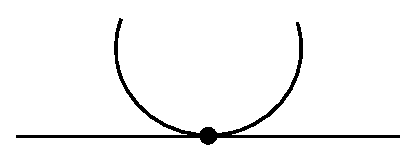
\includegraphics{figure/fig1.eps}
\end{figure}
By\pageoriginale this we mean the ind-object $X$ obtained as the limit
$$
X_{1}\to X_{2}\to\ldots\to X_{n}\to\ldots
$$
where $X_{n}$ is the locus in the plane of
$$
y(y-x^{n})=0
$$
and the map $X_{n}\to X_{n+1}$ sends
$$
(x,y)\mapsto (x,xy).
$$
We take $X$ as ind-object on the category of affine $S$-schemes. Thus by definition
\setcounter{equation}{3}
\begin{equation}
\Hom (Z,X)=\varinjlim\limits_{i}\Hom (Z,X_{i})\label{art02-eq5.4}
\end{equation}
for any {\em affine} $S$-scheme $Z$. For arbitrary $Z$, a map $Z\to X$ is given by a compatible set of maps on an affine open covering.
\end{example}

However, if such examples are avoided, then $(X,x,z)$ is essentially unique.

\setcounter{theorem}{4}
\begin{theorem}[Uniqueness]\label{art02-thm5.5}
With the notation of (\ref{art02-thm5.2}), suppose that in addition the universal element $\overline{z}\in F(\overline{A})$ is uniquely determined. Then the triple $(X,x,z)$ is unique up to unique local isomorphism, for the etale topology, at $x$.
\end{theorem}

Suppose for the moment that the functor $F$ considered in (\ref{art02-thm5.2}) is represented by an algebraic space over $S$, and that the map $z_{0}:\Spec k'\to F$ is a monomorphism, so that $z_{0}$ represents a point, (denote it also by $z_{0}$) of $F$ (\ref{art02-defi2.3}). Then it is easily seen that the map
$$
z:X\to F
$$
of (\ref{art02-thm5.2}) is etale (Section \ref{art02-sec2}) at the point $x\in X$. Thus if we replace $X$ by a suitable Zariski open neighborhood of $x$, we obtain an etale neighborhood of $z_{0}$ in $F$.

Now, taking into account the definition (\ref{art02-defi1.3}), the representability of $F$ by an algebraic space will follow from the existence of a covering by etale neighborhoods. Thus it is intuitively clear that one will be able to derive criteria of representability in the category of algebraic spaces from (\ref{art02-thm5.2}), with effective pro-representability as\pageoriginale a starting point. The following is such a criterion. It is proved in a rather formal way from (\ref{art02-thm5.2}).

\begin{theorem}\label{art02-thm5.6}
Let $F$ be a functor \eqref{art02-eq1.1}, with $S=\Spec k$. Then $F$ is represented by a separated (respectively locally separated) algebraic space if and only if the following conditions hold.
\begin{itemize}
\item[{\rm[0]}] $F$ is a sheaf for the etale topology.

\item[{\rm[1]}] $F$ is locally of finite presentation.

\item[{\rm[2]}] $F$ is effectively pro-representable by complete noetherian local rings.

\item[{\rm[3]}] Let $X$ be an $S$-scheme of finite type, and $z_{1}$, $z_{2}\in F(X)$. Then the kernel of the pair of maps
$$
z_{i}:X\to F
$$
is represented by a closed subscheme (resp. a subscheme) of $X$.

\item[{\rm[4]}] Let $R$ be a $k$-geometric discrete valuation ring with field of fractions $K$, and let $A_{K}$ be a finite local $K$-algebra with residue field $K$. Suppose given elements $z_{1}\in F(R)$, $z_{2}\in F(A_{K})$ which induce the same element of $F(K)$. Then there is a finite $R$-algebra $A$, an augmentation $A\to R$, an isomorphism $A_{K}\approx K\otimes_{R}A$, and an element $z\in F(A)$ which induces $z_{1}$, $z_{2}$.

\item[{\rm[5]}] Let $X$ be a scheme of finite type over $k$ and let $z\in F(X)$. The condition that the map $z:X\to F$ be etale is an open condition on $X$.
\end{itemize}
\end{theorem}

\noindent
Here a map $X\to F$ is called {\em etale at} $x\in X$ if for every map $Y\to F$ there is an open neighborhood $U$ of $x$ in $X$ such that the product $\fprod{U}{Y}{F}$ is represented by a scheme etale over $Y$.

Except for \cite{art02-key4}, the conditions are modifications of familiar ones used in previous results of Murre \cite{art02-key27} and Grothendieck \cite{art02-key28}. Note that condition [0] is just the natural one which assures that $F$ extend to a functor on the category of etale schemes.

The result should be taken primarily as a guide, which can be modified in many ways. This is especially true of conditions \cite{art02-key2}-\cite{art02-key5}. They can be rewritten in terms of standard deformation theory. Thus\pageoriginale for instance condition [2] can be revised by writing out the conditions of pro-representability of Schlessinger \cite{art02-key32} and Levelt \cite{art02-key21}, and condition [3] can be rewritten by applying conditions [0]-[5] to the kernel functor in question. Condition [4] is usually quite easy to verify by deformation theory. The condition which is most difficult to verify as it stands is conditions [5], but this too can be interpreted by infinitesimal methods. In fact, condition [5] can sometimes be dispensed with completely. One has

\begin{theorem}\label{art02-thm5.7}
Let $F$ be a functor on $S$-schemes satisfying [0]-[4] of (\ref{art02-thm5.2}). Suppose that the complete local-rings $\overline{A}$ of condition [2] are all geometrically unibranch and free of embedded components (e.g. normal). Then [5] holds as well, i.e. $F$ is representable by an algebraic space.
\end{theorem}

Here are some examples which illustrate the various conditions of (\ref{art02-thm5.6}) and the relations between them. To begin with, all conditions but [3] hold in example (\ref{art02-exam5.3}).

\begin{example}\label{art02-exam5.8}
The ind-object $X$ (cf. \eqref{art02-eq5.4}) obtained by introducing more and more double points into a line:
\begin{figure}[H]
\centering
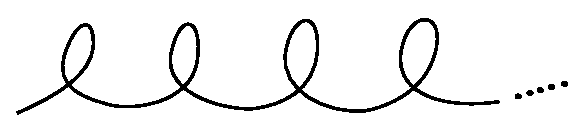
\includegraphics{figure/fig2.eps}
\end{figure}
Neither condition [3] nor [5] hold.
\end{example}

\begin{example}\label{art02-exam5.9}
The ind-object $X$ (cf. \eqref{art02-eq5.4}) obtained as union
\begin{figure}[H]
\centering
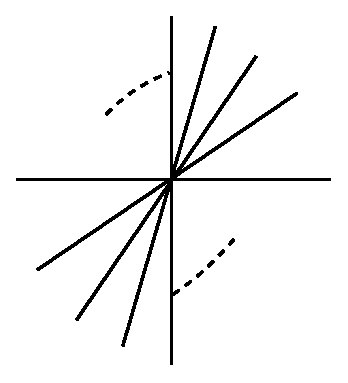
\includegraphics{figure/fig3.eps}
\end{figure}
of\pageoriginale more and more lines through the origin in the plane.
\end{example}

All conditions hold except that in condition [2] the functor is not effectively pro-representable at the origin. Its formal moduli there exist however; they are those of the plane.

\begin{example}\label{art02-exam5.10}
The ind-object $X$ (cf. \eqref{art02-eq5.4}) obtained by adding more and more lines crossing a given line at distinct points.
\begin{figure}[H]
\centering
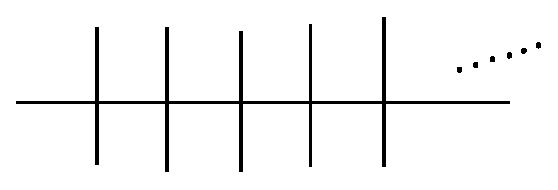
\includegraphics{figure/fig4.eps}
\end{figure}
All conditions but [5] hold.
\end{example}

\begin{example}\label{art02-exam5.11}
The object $X$ is the union of the two schemes $X_{1}=\Spec k[x,y][1/x]$ and $X_{2}=\Spec k[x,y]/(y)$ (the $x$-axis) in the $(x,y)$-plane.
\begin{figure}[H]
\centering
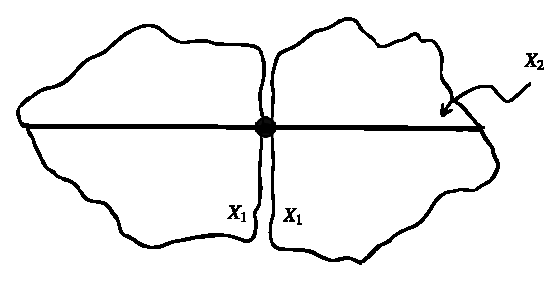
\includegraphics{figure/fig5.eps}
\end{figure}
It is viewed as the following sub-object of the $(x,y)$-plane : A map $f:Z\to \Spec k[x,y]$ represents a map to $X$ if there is an open covering $Z=Z_{1}\cup Z_{2}$ of $Z$ such that the restriction of $f$ to $Z_{i}$ factors through $X_{i}$. In this example, all conditions but [4] hold.
\end{example}

\section{Applications}\label{art02-sec6}
\pageoriginale

Our first application is to Hilbert schemes. We refer to \cite{art02-key12} for the definitions and elementary properties. Recall that Grothendieck \cite{art02-key12} has proved the existence and (quasi)-projectivity of Hilbert schemes $\Hilb X/S$, $\Quot F/X/S$, etc..., when $X$ is (quasi)-projective over $S$. Moreover, Douady \cite{art02-key9} showed their existence as analytic spaces when $X\to S$ is a morphism of analytic spaces. Now if $X$ is not projective over $S$, one can not expect $\Hilb X/S$ to be a scheme, in general. For, consider the example of Hironaka \cite{art02-key16} of a nonsingular variety $X$ over a field and admitting a fixed point free action of $\bfZ/2$ whose quotient $Y$ is not a scheme (though it has a structure of algebraic space). Clearly $Y$ is the sub-object of $\Hilb X/S$ which parametrizes the pairs of points identified by the action, whence $\Hilb X/S$ is not a scheme, by (\ref{art02-coro3.4}). Thus it is natural to consider the problem in the context of etale algebraic spaces.

\begin{theorem}\label{art02-thm6.1}
Let $f:X\to S$ be a morphism locally of finite type of noetherian schemes over a field $k$. Let $F$ be a coherent sheaf on $X$. Then $\Quot F/X/S$ is represented by a locally separated algebraic space over $S$. It is separated if $f$ is. In particular, $\Hilb X/S$ is represented by such an algebraic space.
\end{theorem}

\noindent
Assuming that the cohomology theory for algebraic spaces goes through as predicted, one will be able to replace $f$ above by a morphism of algebraic spaces over $S$, and will thus obtain an assertion purely in that category\footnote{These results are now available, cf. Knutson, op. cit.}. 

Next, we consider the case of relative Picard schemes (cf. \cite{art02-key13} for definitions) for proper maps $f:X\to S$. An example of Mumford (\cite{art02-key13} VI) shows that $\Pic X/S$ is in general not a scheme if the geometric fibres of $f$ are reducible. The following result is proved from (\ref{art02-thm5.6}) using the general techniques of \cite{art02-key13}. The fact that condition [3] of (\ref{art02-thm5.6}) holds for $\Pic X/S$ had been proved previously by Raynaud \cite{art02-key30}.

\begin{theorem}\label{art02-thm6.2}
Let $f:X\to S$ be a proper map of noetherian schemes over a field $k$. Suppose $f$ cohomologically flat in dimension zero, i.e. that\pageoriginale $f_{*}\calO_{X}$ commutes with base change. Then $\Pic X/S$ is represented by a locally separated algebraic space over $S$.
\end{theorem}

\noindent
Again, $f$ can conjecturally be replaced by a morphism of algebraic spaces. When $S=\Spec k$, we obtain from (\ref{art02-thm3.5}) the following theorem of Murre and Grothendieck \cite{art02-key27}.

\begin{theorem}\label{art02-thm6.3}
Let $f:X\to S$ be a proper map of schemes, where $S=\Spec k$. Then $\Pic X/S$ is represented by a scheme.
\end{theorem}

This proof is completely abstract, and is strikingly simple even in the case that $X$ is projective, when one can give a ``classical'' proof using Hilbert schemes. The verification can be reduced to a minimum using the following result. It is the theorem of Murre (\cite{art02-key27}, cf. also \cite{art02-key23}). However, in Murre's formulation there is a condition of existence of a ``module'' for a map of a curve to the group, which is difficult to verify. Here we can just drop that condition completely, and we can remove the hypothesis that the groups be abelian.

\begin{theorem}\label{art02-thm6.4}
Let $F$ be a contravariant functor from ($S$-schemes) to (groups), where $S=\Spec k$. Then $F$ is represented by a scheme locally of finite type over $k$ if and only if
\begin{itemize}
\item[{\rm[0]}] $F$ is a sheaf for the etale topology.

\item[{\rm[1]}] $F$ is locally of finite presentation.

\item[{\rm[2]}] $F$ is effectively pro-representable by a sum of complete noetherian local rings.

\item[{\rm[3]}] Let $X$ be an $S$-scheme of finite type, and $z_{1}$, $z_{2}\in F(X)$.
\end{itemize}

Then the kernel of the pair of maps
$$
z_{i}:X\to F
$$
is represented by a subscheme of $X$.
\end{theorem}

\noindent
As a final application, one obtains the criterion of representability of unramified functors of Grothendieck \cite{art02-key28} in the case that the base $S$ is of finite type over a field. Here again, one can conclude a posteriori that the algebraic space is actually a scheme, by (\ref{art02-thm3.3}). Since\pageoriginale the statement \cite{art02-key28} is rather technical, we will not repeat it here.

\section{Passage to quotient}\label{art02-sec7}

The following result shows that the definition of algebraic space could not be generalized in an essential way by allowing flat equivalence relations. The theorem was proved independently by Raynaud \cite{art02-key30} and me. It shows the strong similarity between algebraic spaces and $Q$-varieties \cite{art02-key24}. However Mumford has pointed out to us that there is a beautiful example due to Holmann (\cite{art02-key19} p.342) of a $Q$-variety which admits no underlying analytic structure.

\begin{theorem}\label{art02-sec7.1}
Let $U$ be an $S$-scheme of finite type and let $i:R\to \fprod{U}{U}{S}$ be a flat equivalence relation. (By this we mean that $i$ is a monomorphism, $R$ is a categorical equivalence relation, and the projection maps $R\rightrightarrows U$ are flat.) Let $X$ be the quotient $U/R$ as sheaf for the fppf topology (cf. \cite{art02-key7} IV). Then $X$ is represented by an algebraic space over $S$. It is separated (resp. locally separated) if $i:R\to\fprod{U}{U}{S}$ is a closed immersion (resp. an immersion). Moreover, $X$ is a universal geometric quotient (cf. \cite{art02-key25}).
\end{theorem}

One wants of course to have more general results on quotients by pre-equivalence relations and by actions of algebraic groups. In the analytic case, there questions have been treated in detail by Holmann \cite{art02-key19} and it seems likely that many of his results have algebraic analogues. Some algebraic results have already been obtained by Seshadri \cite{art02-key33}.

The following is an immediate corollary of (\ref{art02-sec7.1}).

\begin{corollary}\label{art02-coro7.2}
Let $f:Y'\to Y$ be a faithfully flat morphism of algebraic spaces over $S$. Then any descent data for an algebraic space $X'$ over $Y'$ with respect to $f$ is effective.
\end{corollary}

\noindent
Note that because of our definitions, the map $f$ is locally of finite type. We have not proved the result for flat extensions of the base $S'\to S$ which are not of finite type, although in the case that $S$ is of finite type over a field, a proof might be based on (\ref{art02-thm5.6}).

Another\pageoriginale application is to groups in the category of algebraic spaces.

\begin{corollary}\label{coro7.3}
\begin{itemize}
\item[{\rm(i)}] Let $H\to G$ be a morphism of algebraic spaces of groups over $S$, which is a monomorphism. Assume $H$ flat over $S$. Then the cokernel $G/H$ as fppf-sheaf is represented by an algebraic space.

\item[{\rm(ii)}] Let $A$, $B$ be algebraic spaces of abelian groups flat over $S$, and let $E$ be an extension of $B$ by $A$, as fppf-sheaves. Then $E$ is represented by an algebraic space.
\end{itemize}
\end{corollary}

It follows for instance from (i) that one can define groups $\Ext^{q}$ on the category of algebraic spaces of abelian groups flat over $S$, via the definition given in MacLane (\cite{art02-key22} p. 367), taking as distinguished exact sequences the sequences
$$
0\rightarrow A\xrightarrow{i} E\rightarrow B\rightarrow 0
$$
which are exact as $fppf$-sheaves, i.e. such that $i$ is a monomorphism and $B=E/A$. When the base $S$ is not a field, very little is known about these $\Ext^{q}$.

\begin{thebibliography}{99}
\bibitem{art02-key1} \textsc{M. Artin :} {\em Grothendieck topologies,} Harvard University (1962), (mimeographed notes).

\bibitem{art02-key2} \textsc{M. Artin :} On algebraic extensions of local rigns, {\em Rend. di Mat.} 25 (1966), 33-37.

\bibitem{art02-key3} \textsc{M. Artin :} The etale topology of schemes, {\em Proc. Int. Congr. Math. Moscow,} (1966).

\bibitem{art02-key4} \textsc{M. Artin :} Algebraic approximation of structures over complete local rings (to appear).

\bibitem{art02-key5} \textsc{M. Artin and B. Mazur :} On periodic points, {\em Ann. of Math.} 81 (1965), 82-99.

\bibitem{art02-key6} \textsc{M. Artin, A. Grothendieck}\pageoriginale and \textsc{J. L. Verdier :} {\em S\'eminaire de g\'eom\'etrie alg\'ebrique} 1963-64; {\em Cohomologie \'etale des sch\'emas}, Inst. Hautes Etudes Sci. (mimeographed notes).

\bibitem{art02-key7} \textsc{M. Demazure} and \textsc{A. Grothendieck :} {\em S\'eminaire de g\'eom\'etrie alg\'ebrique} 1963-64; {\em Sch\'emas en groupes,} Inst. Hautes Etudes Sci. (mimeographed notes).

\bibitem{art02-key8} \textsc{J. Dieudonn\'e} and \textsc{A. Grothendieck :} {\em \'El\'ements de g\'eom\'etrie alg\'ebrique,} Pub. Math. Inst. Hautes Etudes Sci., Nos. 4-, 1960-.

\bibitem{art02-key9} \textsc{A. Douady :} Le probl\`eme des modules pour les sous-espaces analytiques compacts d'un espace analytique donn\'e, {\em Ann. de l'Inst. Fourier, Grenoble} 16 (1966), 1-98.

\bibitem{art02-key10} \textsc{M. Greenberg :} {\em Rational points in henselian discrete valuation rings,} Pub. Math. Inst. Hautes Etudes Sci., No. 23, 1964.

\bibitem{art02-key11} \textsc{A. Grothendieck :} {\em Technique de descente et th\'eor\`emes d'existence en g\'eom\'etrie alg\'ebrique} II; {\em Le t'eor\`eme d'existence en th\'eorie formelle des modules}, S\'eminaire Bourbaki 12 (1959-60), No. 195 (mimeographed notes). 

\bibitem{art02-key12} \textsc{A. Grothendieck :} {\em Technique de descente et th\'eor\`emes d'existence en g\'eom\'etrie alg\'ebrique} IV; {\em Les sch\'emas de Hilbert}, S\'eminaire Bourbaki 13 (1960-61), No. 221 (mimeographed notes).

\bibitem{art02-key13} \textsc{A. Grothendieck :} {\em Technique de descente et th\'eor\`emes d'existence en g\'eom\'etrie alg\'ebrique} V, VI; {\em Les sch\'emas de Picard,} S\'eminaire Bourbaki 14 (1961-62), Nos 232, 236 (mimeographed notes).

\bibitem{art02-key14} \textsc{A. Grothendieck :} {\em S\'eminaire de g\'eom\'etrie alg\'ebrique} 1960-61, Inst. Hautes Etudes Sci. (mimeographed notes).

\bibitem{art02-key15} \textsc{H. Hironaka :} {\em On the equivalence of singularities} I, Arithmetic algebraic geometry, Proc. Purdue Conf. (1963), Harpers, New York, 1965.

\bibitem{art02-key16} \textsc{H. Hironaka :} An example of a non-K\"ahlerian deformation, {\em Ann. of Math.} 75 (1962), 190---.

\bibitem{art02-key17} \textsc{H. Hironaka :} Formal line bundles along exceptional loci, these {\em Proceedings.}

\bibitem{art02-key18} \textsc{H. Hironaka} and \textsc{H. Rossi :} On the equivalence of imbeddings of exceptional complex spaces, {\em Math. Annalen} 156 (1964), 313-333.

\bibitem{art02-key19} \textsc{H. Holmann :} Komplexe R\"aume mit komplexen Transformationsgruppen, {\em Math. Annalen,} 150 (1963), 327-360.

\bibitem{art02-key20} \textsc{M. Kuranishi :}\pageoriginale On the locally complete families of complex analytic structures, {\em Ann. of Math.} 75 (1962), 536-577.

\bibitem{art02-key21} \textsc{A. H. M. Levelt :} {\em Sur la pro-repr\'esentabilit\'e de certains foncteurs en g\'eom\'etrie alg\'ebrique,} Katholiecke Universit\"eit Nijmegen (1965) (mimeographed notes).

\bibitem{art02-key22} \textsc{S. Maclane :} {\em Homology,} Springer, Berlin, 1963.

\bibitem{art02-key23} \textsc{H. Matsumura} and \textsc{F. Oort :} Representability of group functors and automorphisms of algebraic schemes, {\em Inventiones Math.,} 4 (1967), 1-25.

\bibitem{art02-key24} \textsc{T. Matsusaka :} {\em Theory of $Q$-varieties,} Pub. Math. Soc. Japan No. 8, Tokyo, 1965.

\bibitem{art02-key25} \textsc{D. Mumford :} {\em Geometric invariant theory,} Ergebnisse der Math. Bd. 34, Springer, Berlin, 1965.

\bibitem{art02-key26} \textsc{D. Mumford :} {\em Picard groups of moduli problems,} Arithmetic Algebraic Geometry, Proc. Purdue Conf. (1963), Harpers, New York, 1965.

\bibitem{art02-key27} \textsc{J. P. Murre :} {\em On contravariant functors from the category of preschemes over a field into the category of abelian groups,} Pub. Math. Inst. Hautes Etudes Sci., No. 23, 1964.

\bibitem{art02-key28} \textsc{J. P. Murre :} {\em Representation of unramified functors, Applications,} S\'eminaire Bourbaki, 17 (1964-65) No. 294 (mimeographed notes).

\bibitem{art02-key29} \textsc{J. Nash :} Real algebraic manifolds, {\em Ann. of Math.,} 56 (1952), 405-421.

\bibitem{art02-key30} \textsc{M. Raynaud :} (to appear).

\bibitem{art02-key31} \textsc{P. Samuel :} Algebricit\'e de certains points singuliers algebroides, {\em J. Math. Pures Appl.} 35 (1956), 1-6.

\bibitem{art02-key32} \textsc{M. Schlessinger :} Functions of Artin rings, {\em Trans. Amer. Math. Soc.} 130 (1968), 205-222.

\bibitem{art02-key33} \textsc{C. S. Seshadri :} Some results on the quotient space by an algebraic group of automorphisms, {\em Math. Annalen} 149 (1963), 286-301.

\bibitem{art02-key34} \textsc{A. Weil :} {\em Vari\'et\'es ab\'eliennes et courbes alg\'ebriques,} Hermann, Paris, 1948.
\end{thebibliography}


\bigskip
\noindent
{\small Massachusetts Inst. of Tech.}

\noindent
{\small Cambridge, Mass., U.S.A.}

